\let\negmedspace\undefined
\let\negthickspace\undefined
\documentclass[journal]{IEEEtran}
\usepackage[a5paper, margin=10mm, onecolumn]{geometry}
\usepackage{lmodern} % Ensure lmodern is loaded for pdflatex
\usepackage{tfrupee} % Include tfrupee package

\setlength{\headheight}{1cm} % Set the height of the header box
\setlength{\headsep}{0mm}     % Set the distance between the header box and the top of the text

\usepackage{gvv-book}
\usepackage{gvv}
\usepackage{cite}
\usepackage{amsmath,amssymb,amsfonts,amsthm}
\usepackage{algorithmic}
\usepackage{graphicx}
\usepackage{textcomp}
\usepackage{xcolor}
\usepackage{txfonts}
\usepackage{listings}
\usepackage{enumitem}
\usepackage{mathtools}
\usepackage{gensymb}
\usepackage{comment}
\usepackage[breaklinks=true]{hyperref}
\usepackage{tkz-euclide} 
\usepackage{listings}                                      
\def\inputGnumericTable{}                                 
\usepackage[latin1]{inputenc}                                
\usepackage{color}                                            
\usepackage{array}                                            
\usepackage{longtable}
\usepackage{multicol}
\usepackage{calc}                                             
\usepackage{multirow}                                         
\usepackage{hhline}                                           
\usepackage{ifthen}                                           
\usepackage{lscape}
\begin{document}
	
	\bibliographystyle{IEEEtran}
	\vspace{3cm}
	
	\title{11.16.3.3.3}
	\author{EE24BTECH11030 - KEDARANANDA }
	% \maketitle
	% \newpage
	% \bigskip
	{\let\newpage\relax\maketitle}
	
	\renewcommand{\thefigure}{\theenumi}
	\renewcommand{\thetable}{\theenumi}
	\setlength{\intextsep}{10pt} % Space between text and floats
	
	
	\numberwithin{equation}{enumi}
	\numberwithin{figure}{enumi}
	\renewcommand{\thetable}{\theenumi}
	
	
	\textbf{Question}:\\
	A die is rolled. Find the probability that a number greater than or equal to one will appear.\\
	\textbf{Solution: }\\
	\textbf{Theoretical solution: }\\
	To calculate the probability of rolling a number greater than or equal to one:
	
	\begin{itemize}
		\item A standard die has six faces numbered from 1 to 6.
		\item The total number of possible outcomes is:
		\[
		\text{Total outcomes} = 6.
		\]
		\item The number of outcomes where the number is greater than or equal to one is:
		\[
		\text{Favorable outcomes} = 6.
		\]
		\item The probability is given by:
		\[
		P(\text{Number} \geq 1) = \frac{\text{Favorable outcomes}}{\text{Total outcomes}} = \frac{6}{6} = 1.
		\]
	\end{itemize}
	
	Thus, the probability that a number greater than or equal to one will appear is:
	\[
	\boxed{1}
	\]
	
	\textbf{Computational solution: }\\
	\section*{Z-Transform Computational Method for Die Roll PMF}
	\subsection*{PMF for a Single Die Roll}
	For a single die roll, the probability mass function (PMF) is:
	\[
	P_X(k) =
	\begin{cases}
		\frac{1}{6}, & \text{if } x = 1, 2, 3, 4, 5, 6 \\
		0, & \text{if } x \notin \{1, 2, 3, 4, 5, 6\}
	\end{cases}
	\]
	
	\subsection*{Conditions for PMF}
	A valid PMF must satisfy the following conditions:
	\begin{enumerate}
		\item Non-negativity: \(\forall k, P_X(k) \geq 0\).
		\item Normalization: \(\sum_{k} P_X(k) = 1\).
	\end{enumerate}
	For a single die roll:
	\begin{align}
		P_X(1) + P_X(2) + P_X(3) + P_X(4) + P_X(5) + P_X(6) = 1.
	\end{align}
	Substituting \(P_X(k) = \frac{1}{6}\) for all valid outcomes:
	\begin{align}
		6 \times \frac{1}{6} = 1.
	\end{align}
	
	\subsection*{Z-Transform Expansion}
	The Z-transform for the number rolled is given by:
	\begin{align}
		T(z) = \left( \frac{1}{6}z^1 + \frac{1}{6}z^2 + \frac{1}{6}z^3 + \frac{1}{6}z^4 + \frac{1}{6}z^5 + \frac{1}{6}z^6 \right)
	\end{align}
	where:
	\begin{itemize}
		\item Each term represents the probability of a specific outcome multiplied by its corresponding power of \(z\).
	\end{itemize}
	
	\subsection*{Expansion of \(T(z)\)}
	Simplify the expression:
	\begin{align}
		T(z) = \frac{1}{6}(z^1 + z^2 + z^3 + z^4 + z^5 + z^6).
	\end{align}
	The coefficient of \(z^k\) in \(T(z)\) gives the probability \(P_X(k)\), where \(X\) is the outcome of the die roll.
	
	\subsection*{Probability Mass Function (PMF)}
	The PMF is computed as:
	\begin{align}
		P_X(k) = \frac{1}{6}, \quad k \in \{1, 2, 3, 4, 5, 6\}.
	\end{align}
	
	\subsection*{Computational Steps}
	For each \(k \in \{1, 2, \dots, 6\}\):
	\begin{enumerate}
		\item Compute the binomial coefficient (trivial for single outcomes).
		\item Multiply by \(\frac{1}{6}\) to compute \(P_X(k)\).
	\end{enumerate}
	
	\subsection*{Result for Single Roll}
	The PMF values are:
	\begin{align}
		P_X(1) = \frac{1}{6}, \quad P_X(2) = \frac{1}{6}, \quad \dots, \quad P_X(6) = \frac{1}{6}.
	\end{align}
	
	\subsection*{Conclusion}
	The probability of rolling a number greater than or equal to one is the sum of all PMF values:
	\begin{align}
		P(X \geq 1) = \sum_{k=1}^{6} P_X(k) = \frac{6}{6} = 1.
	\end{align}
	\subsection*{Cumulative Distribution Function (CDF)}
	
	The cumulative distribution function (CDF) \(F(x)\) of a discrete random variable \(X\), representing the outcome of a die roll, is defined as:
	
	\[
	F(x) = P(X \leq x)
	\]
	
	For a die roll with outcomes \(1, 2, 3, 4, 5, 6\), the CDF is:
	
	\[
	F(x) =
	\begin{cases}
		0, & \text{if } x < 1 \\
		\frac{1}{6}, & \text{if } 1 \leq x < 2 \\
		\frac{2}{6}, & \text{if } 2 \leq x < 3 \\
		\frac{3}{6}, & \text{if } 3 \leq x < 4 \\
		\frac{4}{6}, & \text{if } 4 \leq x < 5 \\
		\frac{5}{6}, & \text{if } 5 \leq x < 6 \\
		1, & \text{if } x \geq 6
	\end{cases}
	\]
	
	\begin{figure}[h!]
		\centering
		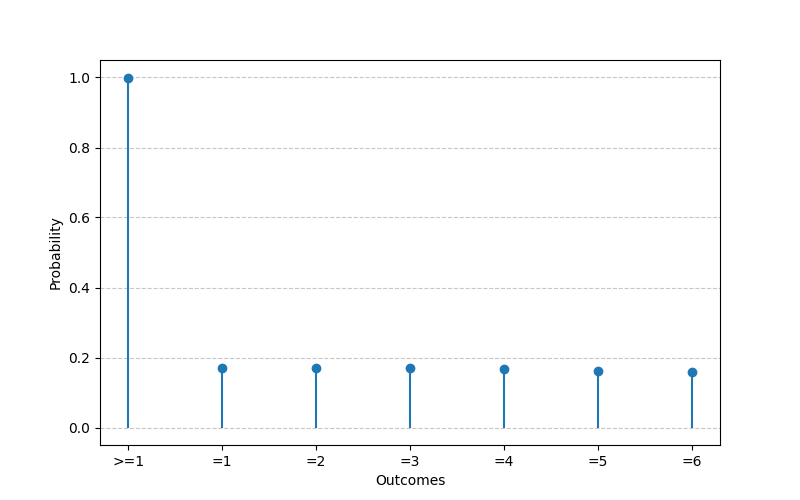
\includegraphics[width=\columnwidth]{figs/Fig.png}
		\label{stemplot}
	\end{figure}
	
\end{document}
